\section{\large Ejercicio 4. Los diferentes tipos de ecuaciones de la recta en $\mathbb{R}^{3}$}

Según su literal seleccionado:
\begin{itemize}
    \item Halle la ecuación vectorial de la recta en $\mathbb{R}^{3}$.
    \item Halle las ecuaciones paramétricas de la recta $\mathbb{R}^{3}$.
    \item Halle las ecuaciones simétricas de la recta $\mathbb{R}^{3}$.
\end{itemize}

Para realizar la comprobación computacional, puede utilizar la herramienta GeoGebra u otra calculadora vectorial. El objetivo de esta comprobación es verificar que las ecuaciones vectorial, paramétrica y simétrica correspondan a la misma recta en $\mathbb{R}^{3}$.

De la recta que pasa por los puntos $P(9,-4,3)$ y $Q(0,2,-3)$.

\textbf{Ecuación vectorial}
\[\vec{r}=P+t\vec{v}\]
\[\vec{v}=(0,2,-3)-(9,-4,3)\]
\[\vec{v}=(-9,6,-6)\]
\[\vec{r}=(9,-4,3)+t(-9,6,-6)\]

\textbf{Verificación en GeoGebra}

\begin{figure}[ht!]
    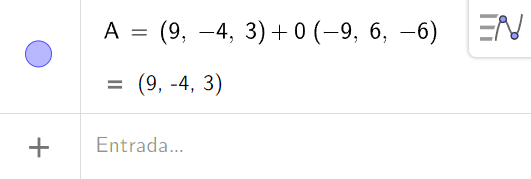
\includegraphics[width=\textwidth]{geogebra3.png}
\end{figure}

\textbf{Ecuaciones paramétricas}
\[(x,y,z)=(9,-4,3)+t(-9,6,-6)\]
\[(x,y,z)=(9,-4,3)+(-9t,6t,-6t)\]
\[(x,y,z)=(9-9t,-4+6t,3-6t)\]

\[
    \begin{cases}
        \begin{array}{l}
            x=9-9t \\
            y=-4+6t \\
            z=3-6t \\
        \end{array}
    \end{cases}
\]

\newpage
\textbf{Verificación en GeoGebra}

\begin{figure}[ht!]
    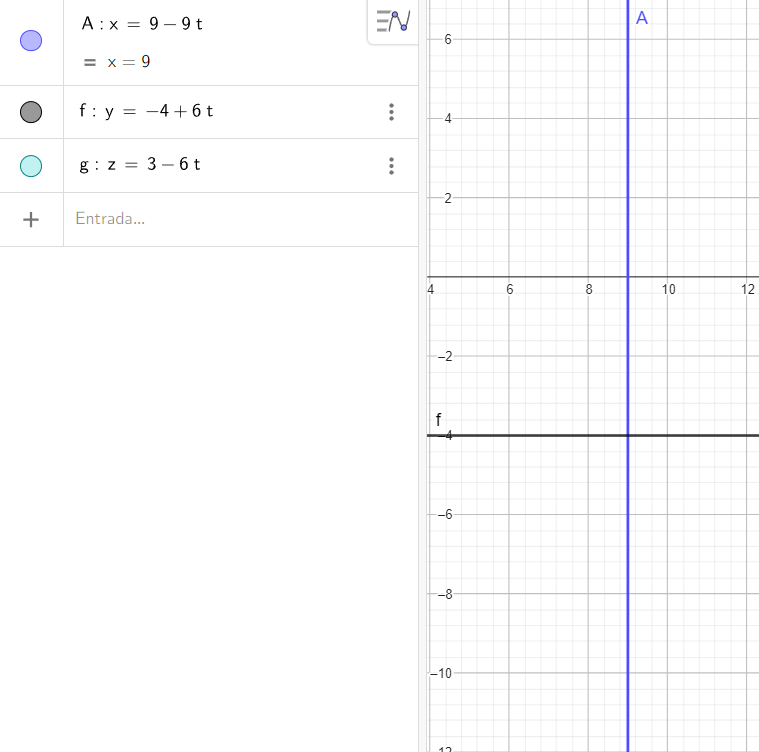
\includegraphics[width=\textwidth, height=400pt]{geogebra4.png}
\end{figure}

\textbf{Ecuaciones simétricas}
\[x=9-9t\]
\[x-9=-9t\]
\[\frac{x-9}{-9}=t\]

\[y=-4+6t\]
\[y+4=+6t\]
\[\frac{y+4}{6}=t\]

\[z=3-6t\]
\[z-3=-6t\]
\[\frac{y-3}{-6}=t\]

\newpage
\textbf{Verificación en GeoGebra}

\begin{figure}[ht!]
    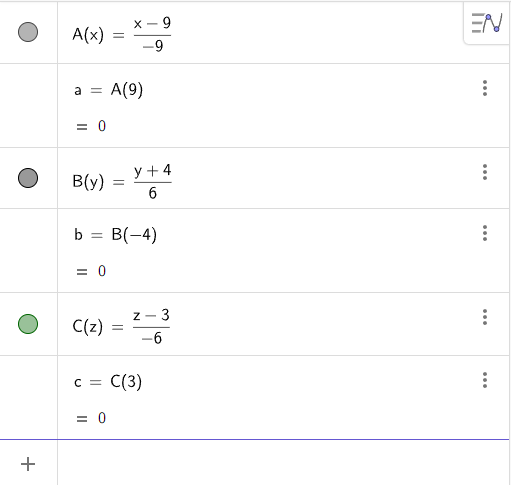
\includegraphics[width=\textwidth, height=400pt]{geogebra5.png}
\end{figure}

\textbf{Respuesta:} En este caso se puede evidenciar que todas las ecuaciones corresponden a la misma recta en $\mathbb{R}^{3}$.